\chapter{معماری
O-RAN
}

ساختاری که در 
\lr{O-RAN}
معرفی شده در 
\ref{fig:oran}
قابل مشاهده است. همان‌طور که می‌بینیم علاوه بر قسمت‌هایی که 
\lr{3GPP}
در ناحیه‌ی دسترسی رادیویی تعبیه کرده بود، قسمت‌های جدیدی هم به آن اضافه شده‌اند 

\begin{figure}[H]
	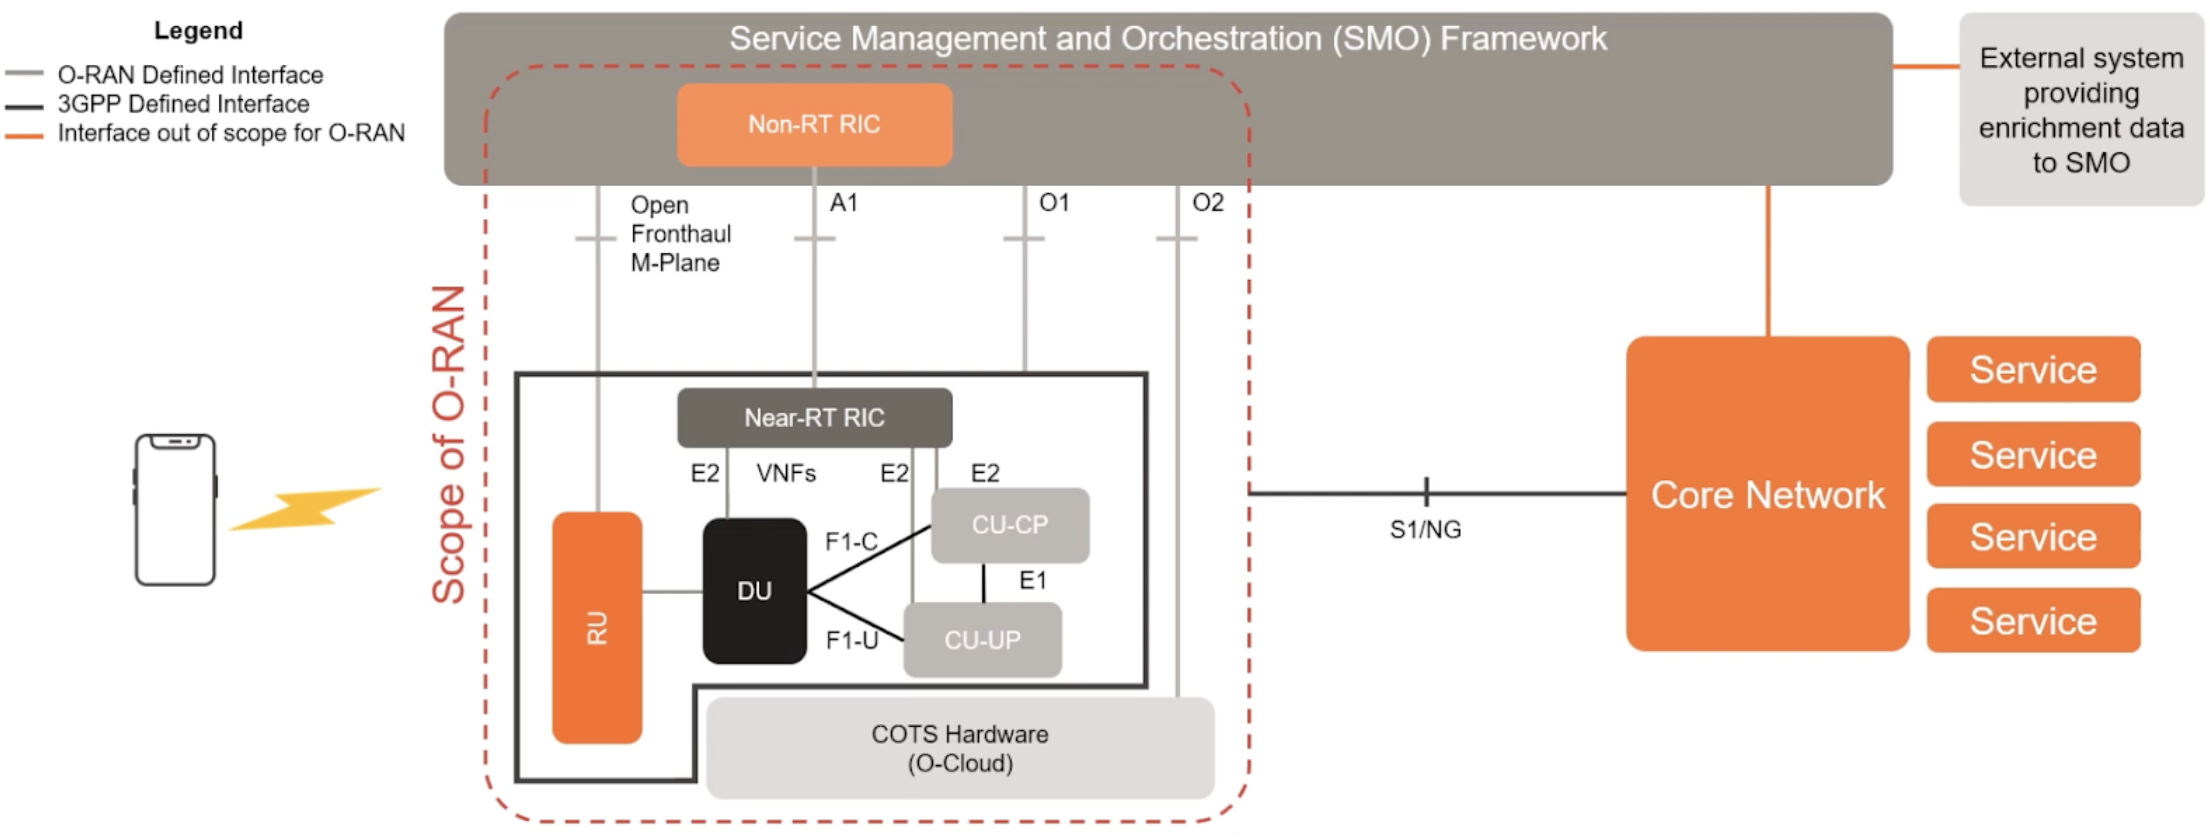
\includegraphics[width=0.85\columnwidth]{Picture/oran.png}
	\centering
	\caption{ساختار کلی شبکه‌های تلفن همراه با
	\lr{O-RAN}}
	\label{fig:oran}
\end{figure}

در 
\ref{fig:oran2} 
تمرکز بر ناحیه‌ی دسترسی رادیویی است و قسمت‌های مختلفی که در
\lr{O-RAN}
در نظر گرفته شده، آورده شده‌اند.

\begin{figure}[H]
	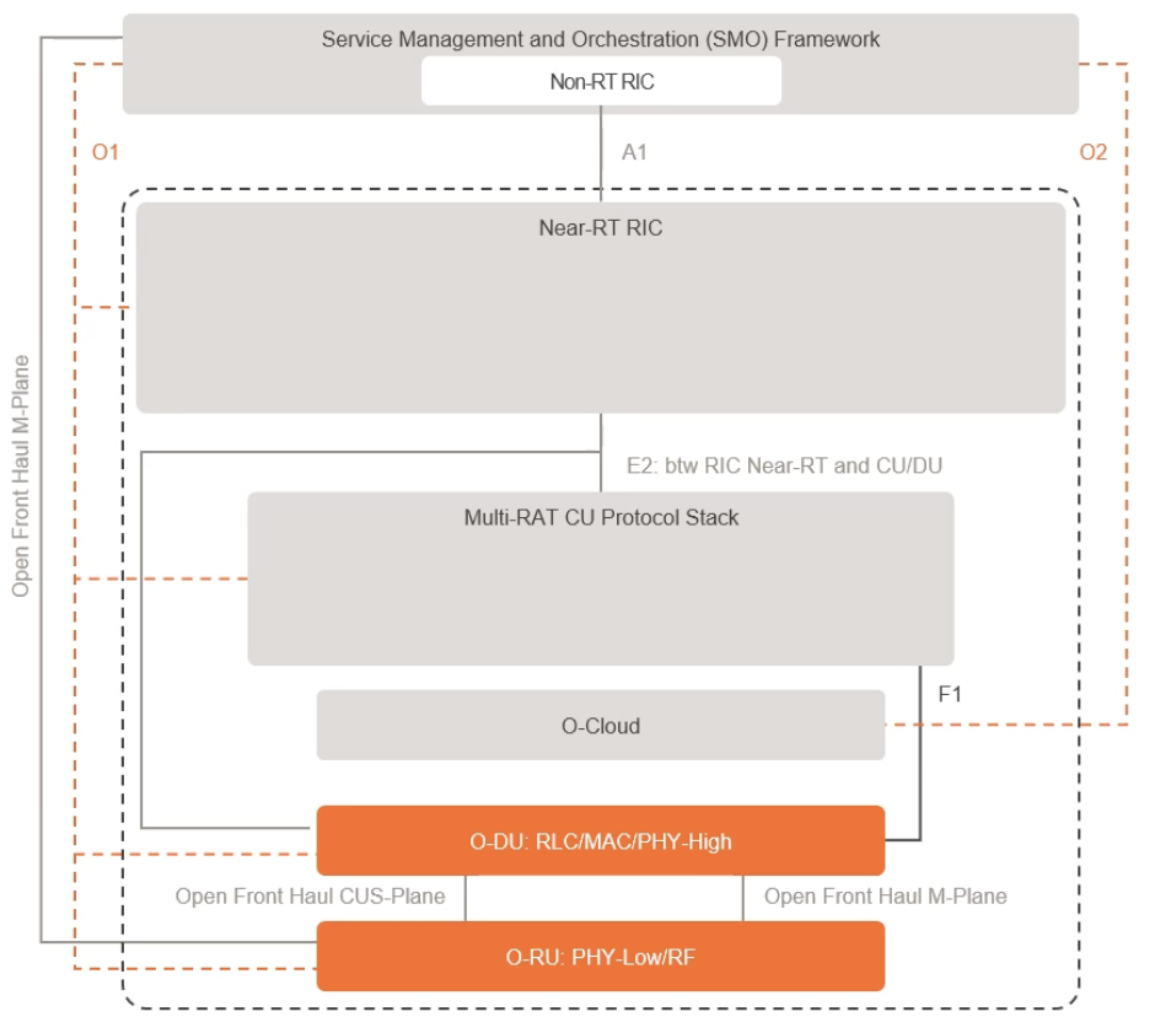
\includegraphics[width=0.85\columnwidth]{Picture/oran2.png}
	\centering
	\caption{اجزای موجود در ناحیه‌ی رادیویی با ساختار
	\lr{O-RAN}}
	\label{fig:oran2}
\end{figure}

می‌بینیم که علاوه بر 
\lr{RU}
\lr{DU}،
و 
\lr{CU}،
قسمت‌های جدیدی مانند 
\lr{Near-Real-Time RIC}
و 
\lr{None-Real-Time RIC}
اضافه شده که این قسمت‌های جدید برای کنترل ناحیه‌ی دسترسی رادیویی به صورت هوشمندانه هستند که در فصل‌های بعدی بررسی شده اند.

در 
\lr{Near-Real-Time RIC}
تمرکز بر کنترل به صورت نزدیک به بلادرنگ است و در 
\lr{None-Real-Time RIC}
کنترل‌های با تاخیر بالاتر از یک ثانیه انجام می‌گیرد. 


